\chapter{संक्षारण और संरक्षण}\label{ch:b2:corrosion}

इस्पात के एक साफ़ टुकड़े पर खारे पानी की एक बूँद छोड़ दीजिए। एक दिन बाद धातु में
बूँद के केंद्र पर गर्त बन जाते हैं, जबकि जंग उसके किनारे के पास एक वलय में बनती है,
जहाँ वायु की ऑक्सीजन घुलती है। लोहा वहाँ घुलता है जहाँ
ऑक्सीजन सबसे कम है, और ऑक्सीजन वहाँ अपचित होती है जहाँ सबसे अधिक है: बूँद
एक ऐसा सेल है जिसे किसी ने नहीं बनाया, जो स्वयं धातु से होकर लघुपथित है। यह
अध्याय संक्षारण को \omterm{def:b2:current-potential-curves:ie-curve}{धारा--विभव वक्रों} पर पढ़ता है, समझाता है कि
खरोंची गई यशदलेपित चादर में जंग क्यों नहीं लगती जबकि खरोंचे गए टिन के डिब्बे में लगती है, और
एक भूमिगत पाइपलाइन के संरक्षण का अभिकल्पन करता है।

\begin{recall}
प्रथम वर्ष का खंड: धातुओं के विभव--pH आरेख और उनके प्रतिरक्षा क्षेत्र,
संक्षारण और \omterm{def:b2:corrosion:passivation}{निष्क्रियण} (``कोई परत रक्षा करती है या नहीं, यह गतिकी का प्रश्न है'')।
\Cref{ch:b2:current-potential-curves}: \omterm{def:b2:current-potential-curves:ie-curve}{धारा--विभव वक्र}, सीमांत
धाराएँ। \Cref{ch:b2:batteries-electrolysis}: \omterm{def:b2:batteries-electrolysis:mixed-potential}{मिश्र विभव}। विद्यालय का
खंड: संक्षारण, जंग, यशदलेपन।
\end{recall}

\begin{omfigure}
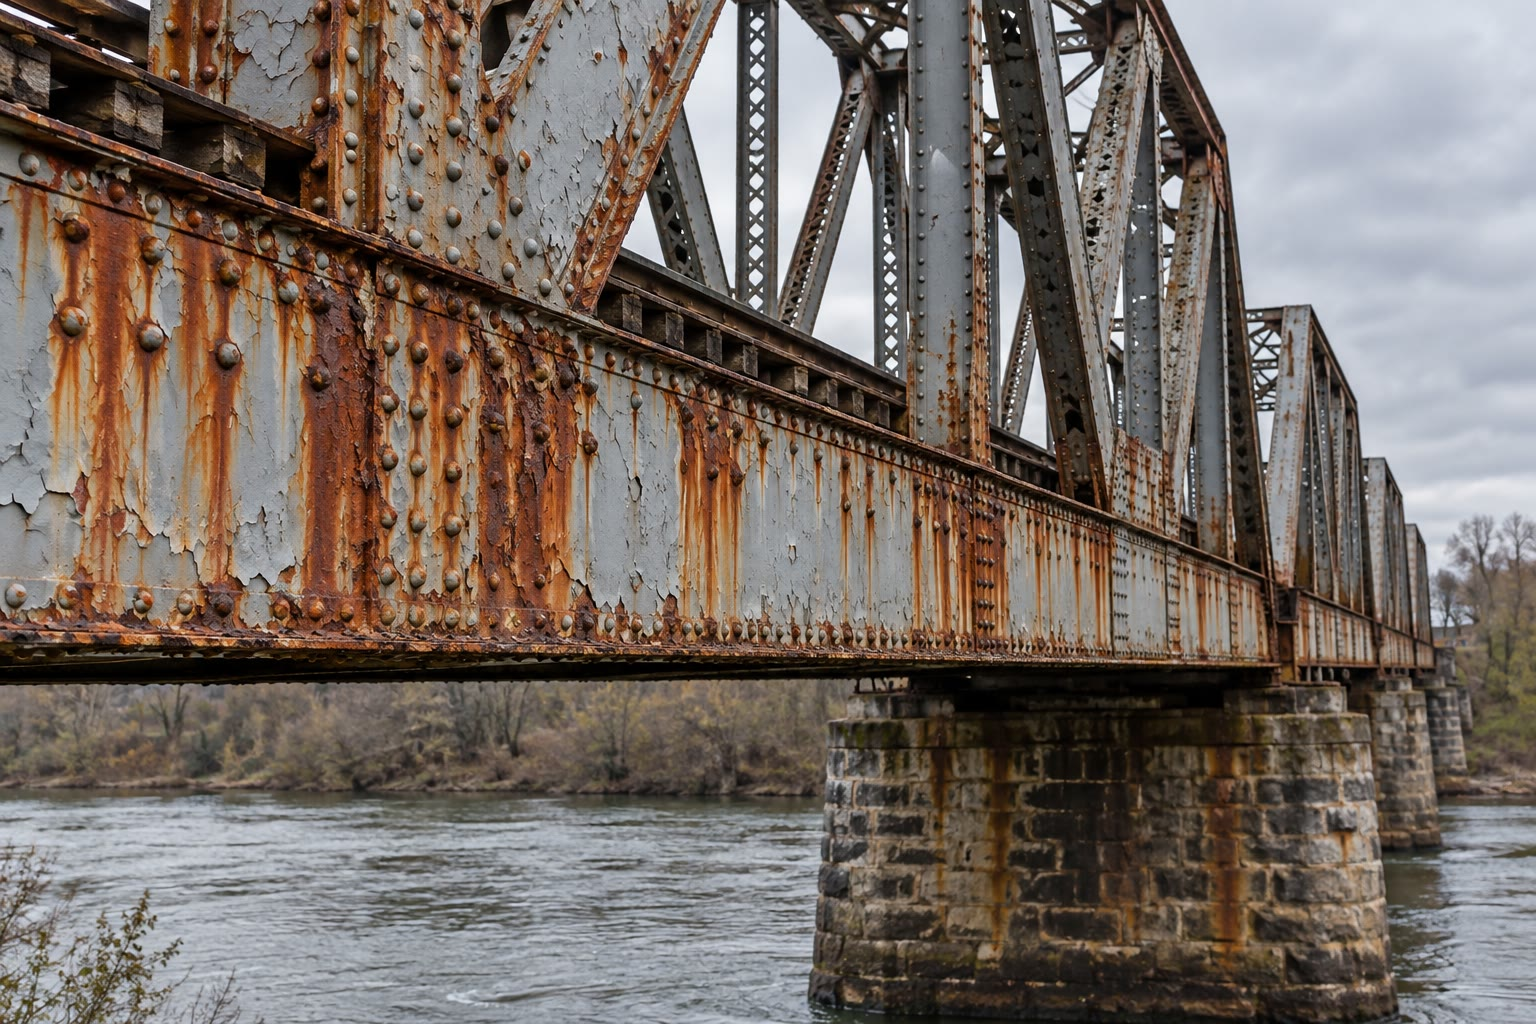
\includegraphics[width=0.62\linewidth]{images/book3/ai/b2-12-rusty-bridge.jpg}

{\small एक पुराना रिवेटदार रेल पुल। जंग की धारियाँ रिवेटों और
जोड़ों से नीचे बहती हैं, जहाँ जल और ऑक्सीजन सबसे देर तक रहते हैं और पेंट सबसे पहले
उखड़ता है।}
\end{omfigure}

\section{लघुपथित सेल के रूप में आर्द्र संक्षारण}

घुली ऑक्सीजन वाले जल में लोहा ऑक्सीकृत होता है, \ce{Fe -> Fe^2+ + 2e-},
और इलेक्ट्रॉन धातु के उसी टुकड़े पर डाइऑक्सीजन के अपचयन द्वारा ग्रहण किए जाते हैं,
\ce{O2 + 2H2O + 4e- -> 4OH-} (अम्ल में \ce{2H+ + 2e- -> H2} द्वारा भी)।
आयरन(II) आयन और हाइड्रॉक्साइड आयन जल में मिलते हैं, और वायु द्वारा आगे का ऑक्सीकरण
उनके अवक्षेप को जंग, एक जलयोजित आयरन(III) ऑक्साइड, में बदल देता है।

\begin{definition}[एकसमान संक्षारण]\label{def:b2:corrosion:uniform}
\emph{एकसमान संक्षारण}\index{एकसमान संक्षारण} किसी धातु का वह संक्षारण है
जिसमें उसका ऑक्सीकरण और ऑक्सीकारक का अपचयन उसकी सतह पर समान रूप से फैले
स्थलों पर होते हैं। \emph{संक्षारण विभव}\index{संक्षारण विभव}
वह \omterm{def:b2:batteries-electrolysis:mixed-potential}{मिश्र विभव} है जो तब धातु लेती है, और
\emph{संक्षारण धारा}\index{संक्षारण धारा} उस विभव पर धातु के ऑक्सीकरण की \omterm{def:b2:current-potential-curves:ie-curve}{ऐनोडी
धारा}।
\end{definition}

\begin{omfigure}
\begin{tikzpicture}
\begin{axis}[omie, width=0.82\linewidth, height=5.6cm, xmin=-1.1, xmax=0.5,
  ymin=-1.6, ymax=1.6, xlabel={$E$}, ylabel={$i$}, clip=true, clip mode=individual,
  axis y line=left]
\addplot[omanodic] table[x=E, y=i] {figdata/out/bachelor-2-ie-curves-i-Fe.dat};
\addplot[omcathodic] table[x=E, y=i] {figdata/out/bachelor-2-ie-curves-i-O2.dat};
\addplot[omcathodic, densely dashed] table[x=E, y=i, y expr=-\thisrow{i}] {figdata/out/bachelor-2-ie-curves-i-O2.dat};
\draw[densely dotted] (axis cs:-0.394,-1.0) -- (axis cs:-0.394,1.0);
\fill (axis cs:-0.394,1.0) circle (1.4pt);
\node[font=\scriptsize, anchor=south east] at (axis cs:-0.40,1.02) {$i_{\text{संक्षारण}}$};
\node[font=\scriptsize, anchor=north west] at (axis cs:-0.39,-0.03) {$E_{\text{संक्षारण}}$};
\node[font=\scriptsize, omThm, anchor=west] at (axis cs:-0.35,1.4) {\ce{Fe} $\to$ \ce{Fe^2+}};
\node[font=\scriptsize, omDef, anchor=north west] at (axis cs:-0.75,-1.05) {\ce{O2} $\to$ \ce{OH-}, विसरण पठार};
\end{axis}
\end{tikzpicture}

{\small वातित उदासीन जल में लोहे का एवांस आरेख (मॉडल वक्र)।
डाइऑक्सीजन का कैथोडी वक्र ऊपर की ओर परावर्तित करके भी खींचा गया है (खंडित): \omterm{def:b2:corrosion:uniform}{संक्षारण
विभव} वहाँ है जहाँ वह लोहे के ऐनोडी वक्र से मिलता है। चूँकि वहाँ
डाइऑक्सीजन का अपचयन अपने विसरण पठार तक पहुँच चुका है, \omterm{def:b2:corrosion:uniform}{संक्षारण
धारा} ऑक्सीजन की \omterm{def:b2:current-potential-curves:limiting-current}{सीमांत धारा} के बराबर है: जल को विलोडित या वातित करने से
लोहा तेज़ी से संक्षारित होता है।}
\end{omfigure}

\begin{proposition}[संक्षारण दर]\label{prop:b2:corrosion:rate}
मोलर द्रव्यमान $M$ और घनत्व $\rho$ वाली धातु, जो प्रति परमाणु $n$ इलेक्ट्रॉनों के साथ
\omterm{def:b2:corrosion:uniform}{संक्षारण धारा} घनत्व $j_{\text{संक्षारण}}$ (प्रति इकाई क्षेत्रफल धारा) के अंतर्गत ऑक्सीकृत होती है,
प्रति इकाई क्षेत्रफल और समय द्रव्यमान $j_{\text{संक्षारण}}M/(nF)$ खोती है, अर्थात्
यह मोटाई:
\[
  \frac{de}{dt} = \frac{j_{\text{संक्षारण}}\,M}{nF\rho} .
\]
\end{proposition}

\begin{proof}
\cref{prop:b2:current-potential-curves:current-rate} से \omterm{def:b2:current-potential-curves:ie-curve}{ऐनोडी धारा}
घनत्व $j_{\text{संक्षारण}}$ प्रति इकाई क्षेत्रफल और समय धातु के $j_{\text{संक्षारण}}/(nF)$ मोल ऑक्सीकृत करता है;
द्रव्यमान के लिए $M$ से गुणा कीजिए और मोटाई के लिए $\rho$ से भाग दीजिए।
\end{proof}

\begin{example}[\qty{10}{\micro A/cm^2} पर लोहा]\label{ex:b2:corrosion:rate}
$j = \qty{0.10}{A/m^2}$, $M = \qty{55.845}{g/mol}$, $n = 2$, $\rho =
\qty{7.87}{g/cm^3}$ के साथ: $de/dt = 0.10 \times 55.845/(2 \times 96\,485 \times 7.87
\times 10^6) = \qty{3.7e-12}{m/s}$, अर्थात् प्रति वर्ष \qty{0.12}{mm}।
% ledger: aw:Fe, rho:Fe, const:F
\end{example}

\section{विभेदी संक्षारण}

\begin{definition}[विभेदी संक्षारण]\label{def:b2:corrosion:differential}
\emph{विभेदी संक्षारण}\index{विभेदी संक्षारण} ऐसा संक्षारण है जिसमें
ऐनोडी और कैथोडी स्थल अलग-अलग होते हैं, और धातु ऐनोडी स्थलों पर
वरीयता से ऑक्सीकृत होती है। यह \emph{गैल्वेनी
संक्षारण}\index{गैल्वेनी संक्षारण} है जब विद्युत संपर्क में दो भिन्न धातुएँ
एक ही विद्युत-अपघट्य साझा करती हैं, और \emph{विभेदी
वातन}\index{विभेदी वातन} जब एक धातु भिन्न ऑक्सीजन मात्राओं वाले जलों के
संपर्क में होती है।
\end{definition}

\begin{proposition}[संपर्क में दो धातुएँ]\label{prop:b2:corrosion:galvanic}
जब विद्युत संपर्क में दो धातुएँ एक ही वातित जल में डूबी होती हैं, तो वे
एक ही \omterm{def:b2:batteries-electrolysis:mixed-potential}{मिश्र विभव} लेती हैं। जिस धातु का \omterm{def:b2:corrosion:uniform}{संक्षारण विभव} कम है, वह
ऐनोड बनती है और अकेले की तुलना में तेज़ी से संक्षारित होती है; दूसरी कैथोड बनती है,
जिस पर डाइऑक्सीजन अपचित होती है, और वह संरक्षित रहती है।
\end{proposition}

\begin{proof}
नगण्य प्रतिरोध वाले चालक से जुड़ी दोनों धातुएँ
एक ही विभव पर होती हैं, जहाँ सभी ऐनोडी धाराओं का योग सभी
कैथोडी धाराओं के योग के ऋण के बराबर होता है। कम उत्कृष्ट धातु का ऐनोडी वक्र पहले उठता है;
सामान्य विभव पर वह लगभग पूरी \omterm{def:b2:current-potential-curves:ie-curve}{ऐनोडी धारा} वहन करता है, और
ऑक्सीजन पूरी गीली सतह पर अपचित होती है, अधिक उत्कृष्ट धातु सहित,
जिसकी अपनी \omterm{def:b2:current-potential-curves:ie-curve}{ऐनोडी धारा} वहाँ नगण्य है।
\end{proof}

\begin{omfigure}
\begin{tikzpicture}
\begin{axis}[omie, width=0.82\linewidth, height=5.6cm, xmin=-1.1, xmax=0.5,
  ymin=-2.4, ymax=2.4, xlabel={$E$}, ylabel={$i$}, clip=true, clip mode=individual,
  axis y line=left]
\addplot[omanodic] table[x=E, y=i] {figdata/out/bachelor-2-ie-curves-i-Fe.dat};
\addplot[omanodic, densely dashed] table[x=E, y=i] {figdata/out/bachelor-2-ie-curves-j-Zn.dat};
\addplot[omcathodic] table[x=E, y=i] {figdata/out/bachelor-2-ie-curves-i-O2.dat};
\addplot[omcathodic, densely dashed] table[x=E, y=i] {figdata/out/bachelor-2-ie-curves-j-O2Cu.dat};
\fill (axis cs:-0.394,1.0) circle (1.4pt);
\fill (axis cs:-0.794,1.0) circle (1.4pt);
\fill (axis cs:-0.366,2.0) circle (1.4pt);
\draw[densely dotted] (axis cs:-1.1,1.0) -- (axis cs:-0.394,1.0);
\draw[densely dotted] (axis cs:-1.1,2.0) -- (axis cs:-0.366,2.0);
\node[font=\scriptsize, anchor=south west] at (axis cs:-0.38,0.95) {अकेला लोहा};
\node[font=\scriptsize, anchor=west] at (axis cs:-0.35,2.0) {लोहा + ताँबा};
\node[font=\scriptsize, anchor=south east] at (axis cs:-0.80,1.05) {लोहा + ज़िंक};
\node[font=\scriptsize, omThm, anchor=north west] at (axis cs:-0.98,0.75) {ज़िंक};
\node[font=\scriptsize, omThm, anchor=north west] at (axis cs:-0.55,0.75) {लोहा};
\node[font=\scriptsize, omDef, anchor=north east] at (axis cs:0.45,-2.05) {लोहा + ताँबा पर \ce{O2}};
\node[font=\scriptsize, omDef, anchor=north east] at (axis cs:0.45,-1.05) {लोहे पर \ce{O2}};
\end{axis}
\end{tikzpicture}

{\small अन्य धातुओं से युग्मित लोहा (मॉडल वक्र)। ज़िंक के साथ सामान्य
विभव वहाँ तक गिरता है जहाँ ज़िंक \omterm{def:b2:current-potential-curves:ie-curve}{ऐनोडी धारा} वहन करता है: लोहा संरक्षित रहता है,
ज़िंक संक्षारित होता है। ताँबे के साथ ऑक्सीजन के लिए कैथोडी क्षेत्रफल दुगुना हो जाता है: लोहे की
\omterm{def:b2:corrosion:uniform}{संक्षारण धारा} भी दुगुनी हो जाती है।}
\end{omfigure}

\begin{proposition}[विभेदी वातन]\label{prop:b2:corrosion:aeration}
भिन्न ऑक्सीजन मात्राओं वाले जलों के संपर्क में किसी धातु पर, कम वातित
क्षेत्र ऐनोडी होता है और संक्षारित होता है; बेहतर वातित क्षेत्र कैथोडी होता है।
\end{proposition}

\begin{proof}
जहाँ ऑक्सीजन की मात्रा अधिक है, वहाँ \ce{O2}/\ce{OH-} युग्म का नेर्न्स्ट विभव
ऊँचा और \omterm{def:b2:current-potential-curves:limiting-current}{सीमांत धारा} बड़ी होती है: कैथोडी वक्र ऊपर रहता है
और दूर तक पहुँचता है। धातु, एक ही चालक होने के कारण, एक विभव पर स्थिर होती है;
वातित क्षेत्र में उपलब्ध बड़ी \omterm{def:b2:current-potential-curves:ie-curve}{कैथोडी धारा} को किसी \omterm{def:b2:current-potential-curves:ie-curve}{ऐनोडी धारा} से संतुलित होना
होता है, जो वहाँ बहती है जहाँ धातु ऑक्सीजन अपचयन की कम
प्रतिस्पर्धा के साथ ऑक्सीकृत हो सकती है, अर्थात् कम वातित क्षेत्र में। ऑक्सीकरण
वहीं केंद्रित होता है।
\end{proof}

\begin{omfigure}
\begin{tikzpicture}[font=\small, >={Stealth}]
  \fill[black!20] (-4.2,-0.7) rectangle (4.2,0);
  \node[font=\scriptsize] at (3.7,-0.35) {इस्पात};
  \fill[omDef!15] (-3.4,0) .. controls (-2.9,2.2) and (2.9,2.2) .. (3.4,0) -- cycle;
  \draw[thick, omDef] (-3.4,0) .. controls (-2.9,2.2) and (2.9,2.2) .. (3.4,0);
  \fill[omProp!80] (-0.7,0) arc[start angle=180, end angle=360, x radius=0.7, y radius=0.22] -- cycle;
  \fill[brown!70!black] (-1.9,0.12) ellipse (0.45 and 0.11);
  \fill[brown!70!black] (1.9,0.12) ellipse (0.45 and 0.11);
  \node[font=\scriptsize, align=center] at (0,2.45) {वायु से \ce{O2}};
  \draw[->, thick, omDef] (-1.0,2.25) -- (-2.6,0.35);
  \draw[->, thick, omDef] (1.0,2.25) -- (2.6,0.35);
  \node[font=\scriptsize, align=center, anchor=east] at (-4.1,1.3) {कैथोड\\ (किनारा)};
  \draw[->, thin] (-4.1,1.3) -- (-3.05,0.12);
  \node[font=\scriptsize, align=center, anchor=west] at (4.1,1.3) {जंग का वलय};
  \draw[->, thin] (4.1,1.3) -- (2.3,0.2);
  \draw[->, omThm] (-0.4,-0.3) .. controls (-1.2,-0.5) and (-2.4,-0.5) .. (-3.0,-0.15);
  \draw[->, omThm] (0.4,-0.3) .. controls (1.2,-0.5) and (2.4,-0.5) .. (3.0,-0.15);
  \draw[->, thin] (0,-1.05) -- (0,-0.25);
  \node[font=\scriptsize, anchor=north] at (0,-1.05) {ऐनोड (केंद्र): \ce{Fe -> Fe^2+ + 2e-}};
  \node[font=\scriptsize, omThm, anchor=north] at (0,-1.45) {इलेक्ट्रॉन इस्पात से होकर किनारे तक बहते हैं};
  \node[font=\scriptsize, anchor=north] at (0,-1.85) {कैथोड (किनारा): \ce{O2 + 2H2O + 4e- -> 4OH-}};
\end{tikzpicture}

{\small इस्पात पर एवांस की बूँद, व्यवस्था-रूप। ऑक्सीजन सतह पर घुलती है और
धातु तक अधिकतर बूँद के पतले किनारे के पास पहुँचती है, जो
कैथोड बन जाता है; ऑक्सीजन से वंचित केंद्र ऐनोड है और उसमें गर्त बनते हैं।
आयरन(II) आयन और हाइड्रॉक्साइड आयन बीच में मिलते हैं, जहाँ जंग एक वलय के रूप में
अवक्षेपित होती है।}
\end{omfigure}

यही क्रियाविधि दरारों पर, किसी संरचना के जमाव या
गैस्केट के नीचे वाले भागों पर, और समुद्र में किसी इस्पात खंभे पर जल-रेखा से ठीक नीचे आक्रमण करती है, जहाँ
जल सतह की तुलना में कम वातित होता है।

\begin{method}[संक्षारण का निदान]\label{met:b2:corrosion:diagnose}
\begin{enumerate}
  \item संपर्क में धातुएँ और विद्युत-अपघट्य सूचीबद्ध कीजिए; जाँचिए कि वे
        विद्युत रूप से जुड़ी हैं।
  \item दो धातुओं के लिए, कम \omterm{def:b2:corrosion:uniform}{संक्षारण विभव} वाली (सामान्यतः कम
        मानक विभव वाली) ऐनोड है।
  \item एक धातु के लिए, कम वातित क्षेत्र (दरारें, जमावों के नीचे,
        बूँद की तली) खोजिए: वे ऐनोडी हैं।
  \item दर कैथोडी अभिक्रिया (ऑक्सीजन की आपूर्ति, कैथोड का क्षेत्रफल) से तय होती है:
        बड़े कैथोड पर छोटा ऐनोड तेज़ी से संक्षारित होता है।
\end{enumerate}
\end{method}

\section{निष्क्रियण}

\begin{definition}[निष्क्रियण]\label{def:b2:corrosion:passivation}
\emph{निष्क्रियण}\index{निष्क्रियण} किसी धातु की संक्षारण दर की वह तीव्र
कमी है जो तब होती है जब वह अपने ऑक्साइड की एक पतली, सघन, दृढ़ता से चिपकी परत,
\emph{निष्क्रिय परत}\index{निष्क्रिय परत}, से ढक जाती है, जो उसे
विलयन से अलग करती है। इस अवस्था में धातु को निष्क्रिय कहा जाता है।
\end{definition}

\begin{proposition}[निष्क्रिय पठार]\label{prop:b2:corrosion:passivity}
निष्क्रियणीय धातु का ऐनोडी वक्र उसके \omterm{def:b2:corrosion:uniform}{संक्षारण विभव} से उठता है,
एक शिखर तक पहुँचता है, फिर विभवों के एक परिसर में एक छोटी, लगभग स्थिर निष्क्रिय धारा तक
गिरता है, और उच्च विभवों पर फिर उठता है (पार-निष्क्रिय
क्षेत्र: परत या जल का ऑक्सीकरण)। निष्क्रिय अवस्था स्थानीय रूप से भंग हो सकती है,
उदाहरण के लिए क्लोराइड आयनों के अंतर्गत, जिससे गर्त बनते हैं।
\end{proposition}

\begin{proof}[तर्क]
निम्न \omterm{def:b2:current-potential-curves:overpotential}{अधिविभवों} पर नंगी धातु उत्तरोत्तर तेज़ी से घुलती है। एक
देहली के आगे ऑक्साइड सतह पर स्थायी हो जाता है (विभव--pH आरेख का \omterm{def:b2:corrosion:passivation}{निष्क्रियण}
क्षेत्र) और एक परत बनाता है जिससे आयन केवल धीरे-धीरे गुज़रते हैं: धारा
उस छोटे अभिवाह तक ढह जाती है। उच्च विभवों पर परत स्वयं विलेय स्पीशीज़ में
ऑक्सीकृत होती है, या उस पर जल ऑक्सीकृत होता है। क्लोराइड आयन, छोटे
और प्रबल संकुलक, कमज़ोर बिंदुओं पर परत को घोल सकते हैं, जहाँ नंगी
धातु एक विशाल निष्क्रिय कैथोड के सामने छोटे ऐनोड के रूप में संक्षारित होती है। यहाँ
वक्र की आकृति एक मॉडल है।
\end{proof}

\begin{omfigure}
\begin{tikzpicture}
\begin{axis}[omie, width=0.82\linewidth, height=5.4cm, xmin=-0.7, xmax=1.5,
  ymin=-0.1, ymax=1.3, xlabel={$E$}, ylabel={$i$}, clip=true, clip mode=individual,
  axis y line=left]
\addplot[omanodic] table[x=E, y=i] {figdata/out/bachelor-2-ie-curves-k.dat};
\node[font=\scriptsize, anchor=south] at (axis cs:-0.33,1.0) {सक्रिय};
\node[font=\scriptsize, anchor=south] at (axis cs:0.5,0.06) {निष्क्रिय पठार};
\node[font=\scriptsize, anchor=east] at (axis cs:1.25,0.9) {पार-निष्क्रिय};
\draw[<-, thin] (axis cs:-0.2,0.55) -- (axis cs:0.15,0.7) node[right, font=\scriptsize] {परत बनती है};
\end{axis}
\end{tikzpicture}

{\small निष्क्रियणीय धातु का ऐनोडी वक्र (मॉडल)। धारा, जो नंगी धातु के घुलते समय
बड़ी होती है, \omterm{def:b2:corrosion:passivation}{निष्क्रिय परत} बनने पर ढह जाती है, और पार-निष्क्रिय उठान से पहले
विभवों के एक चौड़े परिसर में छोटी बनी रहती है।}
\end{omfigure}

स्टेनलेस इस्पातों में इतना क्रोमियम होता है कि वे क्रोमियम ऑक्साइड की ऐसी \omterm{def:b2:corrosion:passivation}{निष्क्रिय परत}
बनाते हैं जो वायु में स्वयं भर जाती है; ऐलुमिनियम अपनी ऐलुमिना परत से संरक्षित है, जो
श्रेणी में हाइड्रोजन से बहुत नीचे की धातु को खिड़की के फ़्रेमों और
पेय के डिब्बों के लिए उपयोगी बना देती है। खुली वायु में ताँबा हरा हो जाता है, क्योंकि पैटिना
क्षारकीय ताँबा लवणों की एक परत है जो आगे के आक्रमण को धीमा करती है।

\begin{omfigure}
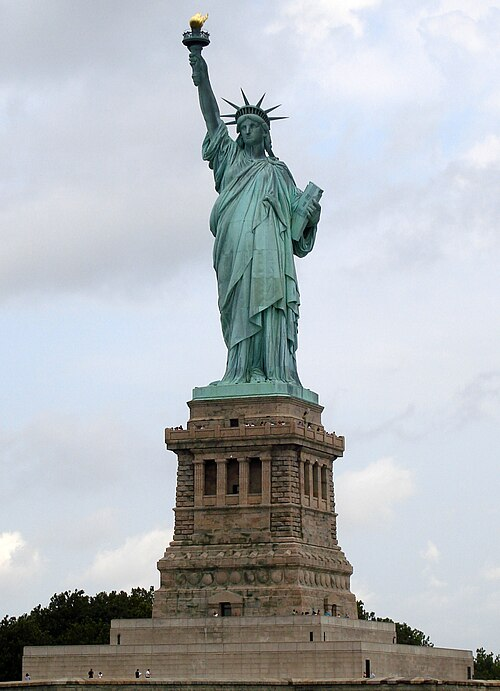
\includegraphics[width=0.32\linewidth]{images/book3/liberty.jpg}

{\small एक सदी से अधिक पुरानी ताँबे की प्रतिमा: पतली ताँबा चादर की उसकी त्वचा
हरी हो गई है, क्षारकीय ताँबा लवणों की पैटिना से ढकी, जो नीचे की धातु की
रक्षा करती है। (छायाचित्र: एलकोबोला, सार्वजनिक अधिकार-क्षेत्र, विकिमीडिया कॉमन्स।)}
\end{omfigure}

\section{संरक्षण}

संक्षारण से लड़ने के उपाय हैं: धातु को जल और ऑक्सीजन से अलग करना (पेंट,
प्लास्टिक, इनैमल, या किसी अन्य धातु की परत), माध्यम को बदलना
(ऑक्सीजन हटाना, धातु पर अधिशोषित होने वाले संदमक मिलाना), या धातु के
विभव को उसके प्रतिरक्षा क्षेत्र में खिसकाना।

\begin{definition}[कैथोडी संरक्षण]\label{def:b2:corrosion:protection}
\emph{कैथोडी संरक्षण}\index{कैथोडी संरक्षण} किसी धातु संरचना का विभव तब तक
घटाता है जब तक उसका ऑक्सीकरण रुक न जाए, उसे किसी सेल का कैथोड बनाकर।
सेल \emph{बलिदानी ऐनोड}\index{बलिदानी ऐनोड} से बनाया जा सकता है,
अर्थात् संरचना से जुड़ी और उसके स्थान पर उपभुक्त होने वाली एक कम उत्कृष्ट धातु (ज़िंक, मैग्नीशियम,
ऐलुमिनियम मिश्रधातुएँ), या किसी जनित्र द्वारा चलाया जा सकता है,
\emph{आरोपित-धारा संरक्षण}\index{आरोपित-धारा संरक्षण} में, जहाँ
ऐनोड तब निकट गड़ा एक अक्रिय इलेक्ट्रोड होता है।
\end{definition}

\begin{proposition}[बलिदानी ऐनोड की आयु]\label{prop:b2:corrosion:anode-life}
द्रव्यमान $m$ और मोलर द्रव्यमान $M$ वाला \omterm{def:b2:corrosion:protection}{बलिदानी ऐनोड}, जो $n$ इलेक्ट्रॉनों के साथ
और दक्षता $\eta$ (धातु का वह अंश जो उपयोगी धारा उत्पन्न करता है, शेष
स्वयं संक्षारित हो जाता है) के साथ ऑक्सीकृत होता है, धारा $I$ इतने समय तक देता है:
\[
  t = \frac{\eta\,m\,nF}{M I} .
\]
\end{proposition}

\begin{proof}
उपयोगी आवेश $\eta\,(m/M)\,nF$ है; धारा से भाग दीजिए।
\end{proof}

\begin{omfigure}
\begin{tikzpicture}[font=\small, >={Stealth}]
  \fill[brown!20] (-4.2,-2.4) rectangle (4.2,0);
  \draw[thick] (-4.2,0) -- (4.2,0);
  \node[font=\scriptsize, anchor=south west] at (-4.2,0) {भूमि};
  \fill[black!40] (-3.5,-1.6) rectangle (3.5,-1.2);
  \node[font=\scriptsize, white] at (0,-1.4) {इस्पात पाइप (कैथोड)};
  % sacrificial anode
  \fill[black!65] (-3.2,-2.3) rectangle (-2.2,-1.95);
  \node[font=\scriptsize, anchor=north] at (-2.7,-2.3) {Mg ऐनोड};
  \draw[thick] (-2.7,-1.95) -- (-2.7,-1.6);
  \draw[->, omProp, thick] (-2.2,-2.12) -- (-1.4,-1.7);
  \node[font=\scriptsize, omProp, anchor=west] at (-1.9,-2.2) {मिट्टी में धारा};
  % impressed current
  \draw[thick, rounded corners] (1.8,0.4) rectangle (3.2,1.2);
  \node[font=\scriptsize] at (2.5,0.8) {दिष्टकारी};
  \fill[black!65] (3.4,-2.3) rectangle (3.9,-1.8);
  \node[font=\scriptsize, anchor=north] at (3.65,-2.3) {अक्रिय ऐनोड};
  \draw[thick] (3.2,0.8) -- (3.65,0.8) -- (3.65,-1.8);
  \draw[thick] (1.8,0.8) -- (1.2,0.8) -- (1.2,-1.2);
  \node[font=\scriptsize, anchor=south] at (3.65,0.85) {$+$};
  \node[font=\scriptsize, anchor=south] at (1.2,0.85) {$-$};
  \node[font=\scriptsize, align=center] at (-2.7,0.8) {बलिदानी ऐनोड};
  \node[font=\scriptsize, align=center] at (2.5,1.55) {आरोपित धारा};
\end{tikzpicture}

{\small भूमिगत पाइप का \omterm{def:b2:corrosion:protection}{कैथोडी संरक्षण}, व्यवस्था-रूप। बाएँ: पाइप से तार द्वारा जुड़ा
मैग्नीशियम ऐनोड उसके स्थान पर संक्षारित होता है। दाएँ: एक दिष्टकारी एक अक्रिय ऐनोड से
मिट्टी से होकर पाइप में धारा चलाता है।}
\end{omfigure}

\begin{omfigure}
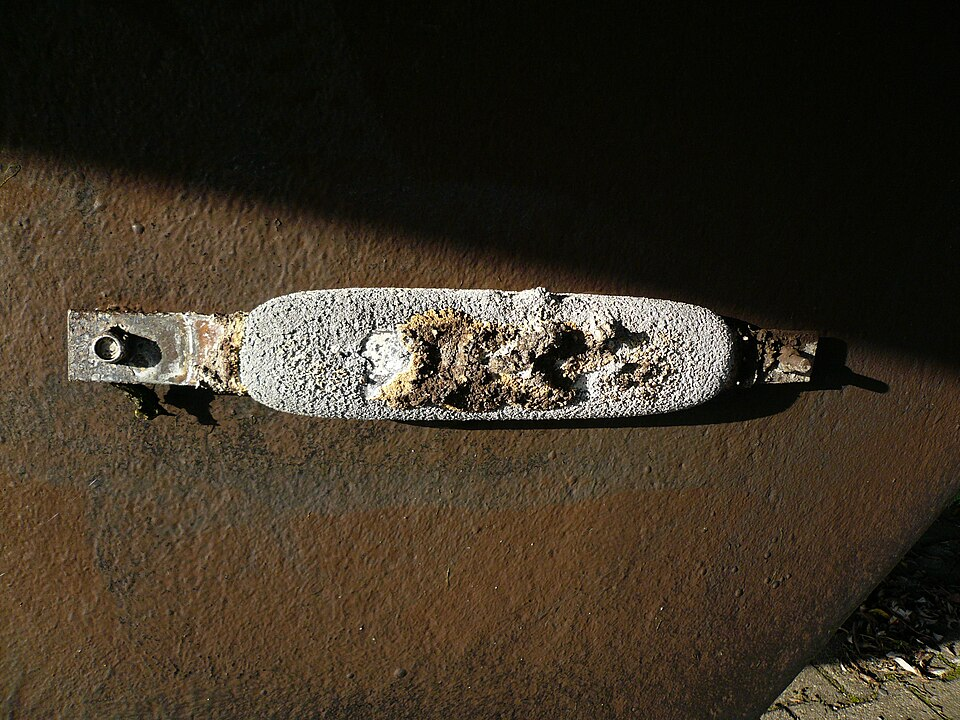
\includegraphics[width=0.5\linewidth]{images/book3/sacrificial-anode.jpg}

{\small एक नाव के इस्पात पेंदे पर बोल्ट से कसा ज़िंक \omterm{def:b2:corrosion:protection}{बलिदानी ऐनोड}, जल में एक
मौसम के बाद: ज़िंक खा लिया गया है, उसके चारों ओर का इस्पात अक्षत है।
(छायाचित्र: त्स्वेर्गेलश्टर्न, CC BY-SA 3.0, विकिमीडिया कॉमन्स।)}
\end{omfigure}

\begin{omfigure}
\begin{tikzpicture}[font=\small, >={Stealth}, scale=1.35]
  \begin{scope}
    \fill[black!25] (0,0) rectangle (4,0.6);
    \fill[gray!55] (0,0.6) rectangle (1.7,0.8); \fill[gray!55] (2.3,0.6) rectangle (4,0.8);
    \fill[omDef!15] (0.8,0.8) .. controls (1.3,1.3) and (2.7,1.3) .. (3.2,0.8) -- (2.3,0.8) -- (2.3,0.6) -- (1.7,0.6) -- (1.7,0.8) -- cycle;
    \node[font=\scriptsize] at (2,-0.3) {यशदलेपित इस्पात (ज़िंक परत)};
    \node[font=\scriptsize, align=center] at (2,1.6) {ज़िंक संक्षारित,\\ इस्पात संरक्षित};
    \draw[->, omThm] (1.4,0.85) -- (1.8,0.65);
  \end{scope}
  \begin{scope}[xshift=5.5cm]
    \fill[black!25] (0,0) rectangle (4,0.6);
    \fill[gray!25] (0,0.6) rectangle (1.7,0.8); \fill[gray!25] (2.3,0.6) rectangle (4,0.8);
    \fill[omDef!15] (0.8,0.8) .. controls (1.3,1.3) and (2.7,1.3) .. (3.2,0.8) -- (2.3,0.8) -- (2.3,0.6) -- (1.7,0.6) -- (1.7,0.8) -- cycle;
    \fill[omProp] (1.75,0.6) rectangle (2.25,0.45);
    \node[font=\scriptsize] at (2,-0.3) {टिन-लेपित इस्पात (टिन परत)};
    \node[font=\scriptsize, align=center] at (2,1.6) {खरोंच में इस्पात संक्षारित,\\ तेज़ी से (छोटा ऐनोड)};
  \end{scope}
\end{tikzpicture}

{\small धातु-लेपन के आर-पार एक खरोंच, व्यवस्था-रूप। ज़िंक, लोहे से कम उत्कृष्ट,
ऐनोड बनता है और उघड़े इस्पात की रक्षा करता है, खरोंच का आकार
चाहे जो हो। टिन, लोहे से अधिक उत्कृष्ट, छोटे इस्पात ऐनोड के चारों ओर एक बड़ा कैथोड
बन जाता है, जो नंगे इस्पात से भी तेज़ी से संक्षारित होता है।}
\end{omfigure}

\begin{method}[संरक्षण का चुनाव]\label{met:b2:corrosion:choose-protection}
\begin{enumerate}
  \item गैल्वेनी युग्मों से बचिए: असमान धातुओं को विद्युत-रोधित कीजिए, या कम
        उत्कृष्ट धातु को बड़ा बनाइए।
  \item लेपन कीजिए: अवरोधी लेप (पेंट, टिन) केवल अक्षत रहने तक रक्षा करता है;
        बलिदानी लेप (ज़िंक) खरोंचे जाने पर भी रक्षा करता है।
  \item मिट्टी या समुद्री जल में किसी संरचना के लिए \omterm{def:b2:corrosion:protection}{कैथोडी संरक्षण} जोड़िए:
        छोटी धाराओं या चालक जल के लिए \omterm{def:b2:corrosion:protection}{बलिदानी ऐनोड},
        लंबी संरचनाओं या प्रतिरोधी मिट्टियों के लिए आरोपित धारा।
  \item अति-संरक्षण मत कीजिए: बहुत कम विभव संरचना पर जल को हाइड्रोजन में
        अपचित करता है, जो लेपों को उखाड़ता है और उच्च-सामर्थ्य
        इस्पातों को भंगुर बना सकता है।
\end{enumerate}
\end{method}

\section{अभ्यास}

\begin{exercise}[$\star$]\label{exo:b2:corrosion:1}
ज़िंक \qty{2.0}{\micro A/cm^2} के धारा घनत्व के अंतर्गत एकसमान रूप से संक्षारित होता है।
प्रति वर्ष उसकी मोटाई की हानि परिकलित कीजिए ($\rho = \qty{7.13}{g/cm^3}$)।
\end{exercise}

\begin{exercise}[$\star$]\label{exo:b2:corrosion:2}
इस्पात के बोल्ट छत पर ताँबे की चादरें थामे हुए हैं। कौन-सी धातु संक्षारित होती है?
इस्पात की चादरों में ज़िंक की कीलों के लिए यही प्रश्न।
\end{exercise}

\begin{exercise}[$\star$]\label{exo:b2:corrosion:3}
इस्पात की दो प्लेटें एक बोल्ट से जुड़ी हैं और समुद्री जल में छोड़ दी गई हैं। संक्षारण कहाँ
केंद्रित होता है, और क्यों?
\end{exercise}

\begin{exercise}[$\star$]\label{exo:b2:corrosion:4}
एक यशदलेपित बाल्टी और एक टिन का डिब्बा, दोनों इस्पात तक खरोंचे गए हैं। किसमें
खरोंच पर जंग लगती है?
\end{exercise}

\begin{exercise}[$\star\star$]\label{exo:b2:corrosion:5}
वातित जल में लोहे के एवांस आरेख पर समझाइए कि जल को विलोडित करने पर, फिर
उसे ऑक्सीजन से मुक्त करने पर \omterm{def:b2:corrosion:uniform}{संक्षारण विभव} और धारा का क्या होता है।
\end{exercise}

\begin{exercise}[$\star\star$]\label{exo:b2:corrosion:6}
\qty{5.0}{kg} का एक ज़िंक ऐनोड एक नाव के पेंदे की \qty{0.10}{A} की धारा से,
90~\% की दक्षता के साथ, रक्षा करता है (अभ्यास के आँकड़े)। वह कितने समय तक
चलता है?
\end{exercise}

\begin{exercise}[$\star\star$]\label{exo:b2:corrosion:7}
100~\% दक्षता पर ज़िंक, मैग्नीशियम और ऐलुमिनियम ऐनोडों द्वारा दिया गया आवेश, ऐम्पियर-घंटे
प्रति किलोग्राम में, और $\Delta_f G^\circ$ (\ce{Zn^2+} $-147.06$, \ce{Mg^2+} $-454.8$,
\ce{Al^3+} $-485$ \unit{kJ/mol}) से उनके युग्मों के मानक विभव परिकलित कीजिए।
सूखी मिट्टियों में मैग्नीशियम को प्राथमिकता क्यों दी जाती है?
\end{exercise}

\begin{exercise}[$\star\star$]\label{exo:b2:corrosion:8}
एक भूमिगत पाइप को \qty{2.0}{A} संरक्षण धारा चाहिए। अक्रिय ऐनोड के भूमि-संस्तर
का मिट्टी के सापेक्ष प्रतिरोध \qty{4.0}{\ohm} है और सेल को अतिरिक्त
\qty{1.5}{V} चाहिए (अभ्यास के आँकड़े)। दिष्टकारी की वोल्टता और प्रति वर्ष
विद्युत ऊर्जा परिकलित कीजिए।
\end{exercise}

\begin{exercise}[$\star\star$]\label{exo:b2:corrosion:9}
समुद्र में एक इस्पात खंभा खड़ा है। समझाइए कि वह जल-रेखा से थोड़ा नीचे
सबसे अधिक क्यों संक्षारित होता है, स्वयं जल-रेखा पर क्यों नहीं।
\end{exercise}

\begin{exercise}[$\star\star\star$]\label{exo:b2:corrosion:10}
निष्क्रिय वक्र से समझाइए कि स्टेनलेस इस्पात वातित जल का प्रतिरोध क्यों करता है परंतु
समुद्री जल में उसमें गर्त क्यों बन सकते हैं, और एक बार आरंभ होने पर गर्त चौड़ा होने के बजाय
गहरा क्यों होता जाता है।
\end{exercise}

\begin{exercise}[$\star\star\star$]\label{exo:b2:corrosion:11}
वातित जल ले जाने वाले इस्पात पाइप पर ताँबे की एक फ़िटिंग कसी है। हर गीली सतह पर
ऑक्सीजन \omterm{def:b2:current-potential-curves:limiting-current}{सीमांत धारा} घनत्व \qty{5}{\micro A/cm^2} है; ताँबा
\qty{20}{cm^2} प्रदान करता है और जोड़ के निकट का इस्पात \qty{2}{cm^2}
(अभ्यास के आँकड़े)। इस्पात की \omterm{def:b2:corrosion:uniform}{संक्षारण धारा} और जोड़ के निकट प्रति वर्ष उसकी
मोटाई की हानि का आकलन कीजिए।
\end{exercise}

\begin{exercise}[$\star\star\star$]\label{exo:b2:corrosion:12}
लोहे के विभव--pH आरेख और जल के वक्रों से समझाइए कि उदासीन जल में किसी संरक्षित
इस्पात संरचना का विभव लगभग \qty{-0.6}{V} से नीचे, परंतु \qty{-1}{V} से बहुत नीचे नहीं,
क्यों रखना चाहिए।
\end{exercise}

\section{समस्या: एक पाइपलाइन का संरक्षण}

\begin{problem}[{सप्ताहांत समस्या --- गीली मिट्टी में नंगे इस्पात पाइप का
संक्षारण, बलिदानी धातु का चुनाव, बीस वर्षों के लिए आवश्यक मैग्नीशियम,
और आरोपित-धारा विकल्प}]
\label{pb:b2:corrosion:1}
\qty{10.0}{km} लंबी और \qty{0.30}{m} व्यास वाली एक इस्पात पाइपलाइन गीली मिट्टी में
गड़ी है। आँकड़े: लोहा $M = \qty{55.845}{g/mol}$, $\rho = \qty{7.87}{g/cm^3}$;
मैग्नीशियम $M = \qty{24.305}{g/mol}$; $\Delta_f G^\circ$ (\unit{kJ/mol}): \ce{Fe^2+}
$-78.90$, \ce{Zn^2+} $-147.06$, \ce{Mg^2+} $-454.8$, \ce{Al^3+} $-485$। अभ्यास के
आँकड़े: इस मिट्टी में नंगे इस्पात का \omterm{def:b2:corrosion:uniform}{संक्षारण धारा} घनत्व \qty{10}{\micro
A/cm^2}; नंगे इस्पात के संरक्षण के लिए अभिकल्पन धारा घनत्व
\qty{20}{mA/m^2}; लेप सतह का 1.0~\% नंगा छोड़ता है; \qty{15}{kg} के
मैग्नीशियम ऐनोड, दक्षता 50~\%; आरोपित धारा के लिए भूमि-संस्तर प्रतिरोध
\qty{5.0}{\ohm}।
% ledger: aw:Fe, rho:Fe, aw:Mg, dfg:Fe2+_ao, dfg:Zn2+_ao, dfg:Mg2+_ao, dfg:Al3+_ao, const:F

\medskip
\noindent\textbf{भाग I --- नंगा पाइप।}
\begin{enumerate}
  \item पाइप पर ऐनोडी और कैथोडी अभिक्रियाएँ लिखिए।
  \item \omterm{def:b2:corrosion:uniform}{संक्षारण धारा} ऑक्सीजन की आपूर्ति से क्यों तय होती है?
  \item प्रति वर्ग मीटर और प्रति वर्ष खोए लोहे का द्रव्यमान परिकलित कीजिए।
  \item प्रति वर्ष दीवार की मोटाई की हानि परिकलित कीजिए।
  \item नंगे पाइप को \qty{8}{mm} की दीवार का आधा खोने में कितना समय लगेगा?
  \item वास्तविक पाइप कुछ बिंदुओं पर उससे पहले क्यों विफल होता है?
\end{enumerate}

\medskip
\noindent\textbf{भाग II --- ऐनोड धातु।}
\begin{enumerate}[resume]
  \item लोहा, ज़िंक, मैग्नीशियम
        और ऐलुमिनियम के युग्मों के मानक विभव परिकलित कीजिए।
  \item कौन-सी धातुएँ \omterm{def:b2:corrosion:protection}{बलिदानी ऐनोडों} के रूप में लोहे की रक्षा कर सकती हैं?
  \item मिट्टियों में ऐलुमिनियम का उपयोग कम क्यों होता है?
  \item उच्च प्रतिरोधकता वाली मिट्टी में ज़िंक की तुलना में मैग्नीशियम को प्राथमिकता क्यों दी जाती है?
  \item प्रति ऐम्पियर और प्रति वर्ष उपभुक्त मैग्नीशियम का द्रव्यमान परिकलित कीजिए।
\end{enumerate}

\medskip
\noindent\textbf{भाग III --- अभिकल्पन।}
\begin{enumerate}[resume]
  \item पाइप की बाहरी सतह परिकलित कीजिए।
  \item लेप द्वारा छोड़ी गई नंगी सतह परिकलित कीजिए।
  \item संरक्षण धारा परिकलित कीजिए।
  \item बीस वर्षों के लिए आवश्यक आवेश परिकलित कीजिए।
  \item आवश्यक मैग्नीशियम का द्रव्यमान परिकलित कीजिए।
  \item कितने ऐनोड चाहिए?
  \item उन्हें एक बिंदु पर गाड़ने के बजाय पाइप के अनुदिश क्यों बाँटा जाता
        है?
\end{enumerate}

\medskip
\noindent\textbf{भाग IV --- आरोपित धारा।}
\begin{enumerate}[resume]
  \item आरोपित-धारा विकल्प का वर्णन कीजिए।
  \item भूमि-संस्तर प्रतिरोध से, इलेक्ट्रोडों के लिए \qty{1.5}{V} जोड़कर,
        दिष्टकारी की वोल्टता का आकलन कीजिए।
  \item प्रति वर्ष प्रयुक्त विद्युत ऊर्जा परिकलित कीजिए।
  \item यदि पाइप का अति-संरक्षण हो तो क्या गड़बड़ होती है?
  \item \qty{1e-6}{mol/L} आयरन(II) सांद्रता लेकर, उदासीन जल में लोहा
        किस विभव से नीचे प्रतिरक्षित है?
  \item बीस वर्षों के लिए आवश्यक मैग्नीशियम ऐनोडों का द्रव्यमान बताइए।
\end{enumerate}
\end{problem}
